\chapter{Low-Level Design}
\label{ch:low-level-design}

This chapter documents the significant functions, their signatures, their inputs
and outputs, and the state they touch. Signatures are reproduced from the source.

\section{\texttt{@expo-snips/core}}

\subsection*{\texttt{renderTemplate(templateStr, context)}}

\begin{lstlisting}[language=JavaScript]
export function renderTemplate(templateStr: string, context: RenderContext): string
\end{lstlisting}

Compiles the template with Handlebars and executes it against the render context.
Compilation happens per call; there is no cache.

\subsection*{\texttt{getFilesForRecipe(recipe, context, resolveFile?)}}

\begin{lstlisting}[language=JavaScript]
export function getFilesForRecipe(
  recipe: ScreenRecipe,
  context: GenerationContext,
  resolveFile?: (file: FileTemplate) => string | null
): Array<{ path: string; content: string }>
\end{lstlisting}

Algorithm:

\begin{enumerate}
  \item For each entry in \texttt{recipe.files}, evaluate \texttt{when} via
        \texttt{matchesCondition}; skip on mismatch.
  \item Resolve the template string with \texttt{resolveTemplateString}: variant
        override, then per-styling override, then \texttt{template}.
  \item If the template is still null and \texttt{templateFile} is set, delegate to
        the optional \texttt{resolveFile} callback (used when templates were not
        inlined).
  \item Skip the entry if no template could be resolved.
  \item Render and append \texttt{\{path, content\}}.
\end{enumerate}

Only \texttt{path} and \texttt{content} are returned; conditions and metadata are
discarded. Consequently two file entries targeting the same path (a common recipe
pattern --- one entry per supported stack) are filtered down to the single entry
whose conditions match.

\subsection*{\texttt{matchesCondition} (private)}

Evaluates five optional predicates in sequence --- styling, router, ui, icons and
typescript --- returning false on the first mismatch. TypeScript comparison is an
exact equality check, so \texttt{typescript: false} matches only JavaScript
generation.

\subsection*{\texttt{buildRenderContext} (private)}

Projects the generation context into the render context by duplicating the option
values at the top level (\texttt{styling}, \texttt{router}, \texttt{ui},
\texttt{icons}, \texttt{typescript}) so templates can be written as
\texttt{\{\#if (eq styling "nativewind")\}} without an options prefix.

\section{\texttt{@expo-snips/cli} --- utilities}

\begin{longtable}{p{4.2cm}p{9.8cm}}
\caption{CLI utility functions}\\
\toprule
\textbf{Function} & \textbf{Behaviour} \\
\midrule

\texttt{detectProject(dir?)} & Reads \texttt{package.json} for four dependency
probes and \texttt{tsconfig.json} for the language flag; returns
\texttt{DetectedProject}. Defaults: ui \texttt{native}, icons \texttt{none},
styling \texttt{stylesheet} when no \texttt{package.json} exists. \\
\texttt{getRegistryBase(override?)} & Returns \texttt{(override || env || "").trim()}
with trailing slashes removed. \\
\texttt{hasLocalRegistry()} & True when the embedded catalog is non-empty. \\
\texttt{getLocalRecipeById(id)} & Map lookup into the embedded catalog. \\
\texttt{fetchJSON<T>(url)} & \texttt{fetch} with a 10-second \texttt{AbortController}
timeout; returns null on non-OK responses. \\
\texttt{resolveRecipeIndex(base?)} & Remote fetch first; falls back to the local
index; reports \texttt{source} as \texttt{"remote"} or \texttt{"local"}. \\
\texttt{getRecipeIndex(base?)} & Index only. \\
\texttt{getRecipeById(id, base?)} & Remote recipe fetch, then embedded lookup. \\
\texttt{getRecipesByIds(ids, base?)} & Parallel resolve, filtering nulls. \\
\texttt{resolveRegistry(url?)} & Calls \texttt{resolveRecipeIndex} and prints a
source message. \\
\texttt{readManifest(dir?)} & Returns \texttt{\{version:1, installs:[]\}} when the file
is absent or unparseable. \\
\texttt{upsertEntry(entry, dir?)} & Replaces the entry matching
(\texttt{recipeId}, \texttt{variant}) or appends. \\
\texttt{updateEntryVersions(entries, dir?)} & Rewrites \texttt{recipeVersion} for
matching entries. \\
\texttt{getPrimitives(recipe, context, root, findRecipe)} & Recursive primitive
resolution with a \texttt{Set} cycle guard; dedupes dependencies. \\
\texttt{installDependencies(deps, devDeps, dir?)} & Detects the package manager and
runs \texttt{add} / \texttt{add -D}. \\
\texttt{writeFiles(files, root)} & \texttt{ensureDir} then \texttt{writeFile} per
file, logging each path. \\
\texttt{diffLines(oldText, newText)} & Builds an $(n+1)\times(m+1)$ LCS table and
walks it to emit add/remove/context hunks. \\
\texttt{printDiff(path, old, new)} & Prints coloured hunks; no output when nothing
changed. \\
\texttt{hasChanges(old, new)} & Strict string inequality. \\
\bottomrule
\end{longtable}

\subsection*{Manifest data structures}

\begin{lstlisting}[language=JavaScript]
interface ManifestOptions { styling: string; router: string; ui: string; icons: string; typescript: boolean; }
interface ManifestEntry { recipeId: string; recipeVersion: string; installedAt: string; options: ManifestOptions; variant?: string; files: string[]; }
interface Manifest { version: number; installs: ManifestEntry[]; }
const MANIFEST_FILENAME = ".expo-snips.json";
\end{lstlisting}

\subsection*{The \texttt{add} command in detail}

\texttt{add.ts} is the longest command and the best illustration of the CLI's
control flow.

\begin{longtable}{p{1.5cm}p{12.3cm}}
\caption{\texttt{add} command steps}\\
\toprule
\textbf{Lines} & \textbf{Step} \\
\midrule

68--70 & Resolve the registry; prepare a \texttt{findRecipe} closure. \\
72--92 & If no id was supplied, list the index in a select prompt; abort with exit
code 1 if empty or cancelled. \\
94--100 & Load the recipe; error with guidance if not found. \\
102 & Detect the project. \\
104--117 & Resolve styling; validate any explicit value; fall back to a detected
value only when the recipe supports it. \\
119--159 & Resolve router, ui and icons with the same pattern, including the
``single supported value'' shortcut. \\
161--165 & Resolve language; warn when a TypeScript recipe is generated as
JavaScript. \\
167--200 & Prompt for any option still unresolved, offering only supported values
and preselecting the detected one. \\
202--214 & Enforce the shadcn constraints. \\
216--222 & Build the generation context with \texttt{projectRoot: process.cwd()}. \\
224--230 & Render; error when no files matched. \\
232--238 & Announce the recipe and the effective option values. \\
238 & Write files. \\
240--256 & Resolve and write shadcn primitives; merge their dependencies; report
skipped files. \\
258--260 & Install dependencies unless \texttt{--no-install} was given. \\
262--272 & Upsert the manifest entry. \\
274--278 & Print success and next steps. \\
\bottomrule
\end{longtable}

\textbf{Observation.} Styling resolution appears twice: lines 111--117 compute a
detected styling, and lines 167--173 recompute the same value before prompting.
The duplicate is harmless but redundant (recorded in
Chapter~\ref{ch:technical-debt}).

\section{The recipe primitive graph}

\begin{figure}[H]
\centering
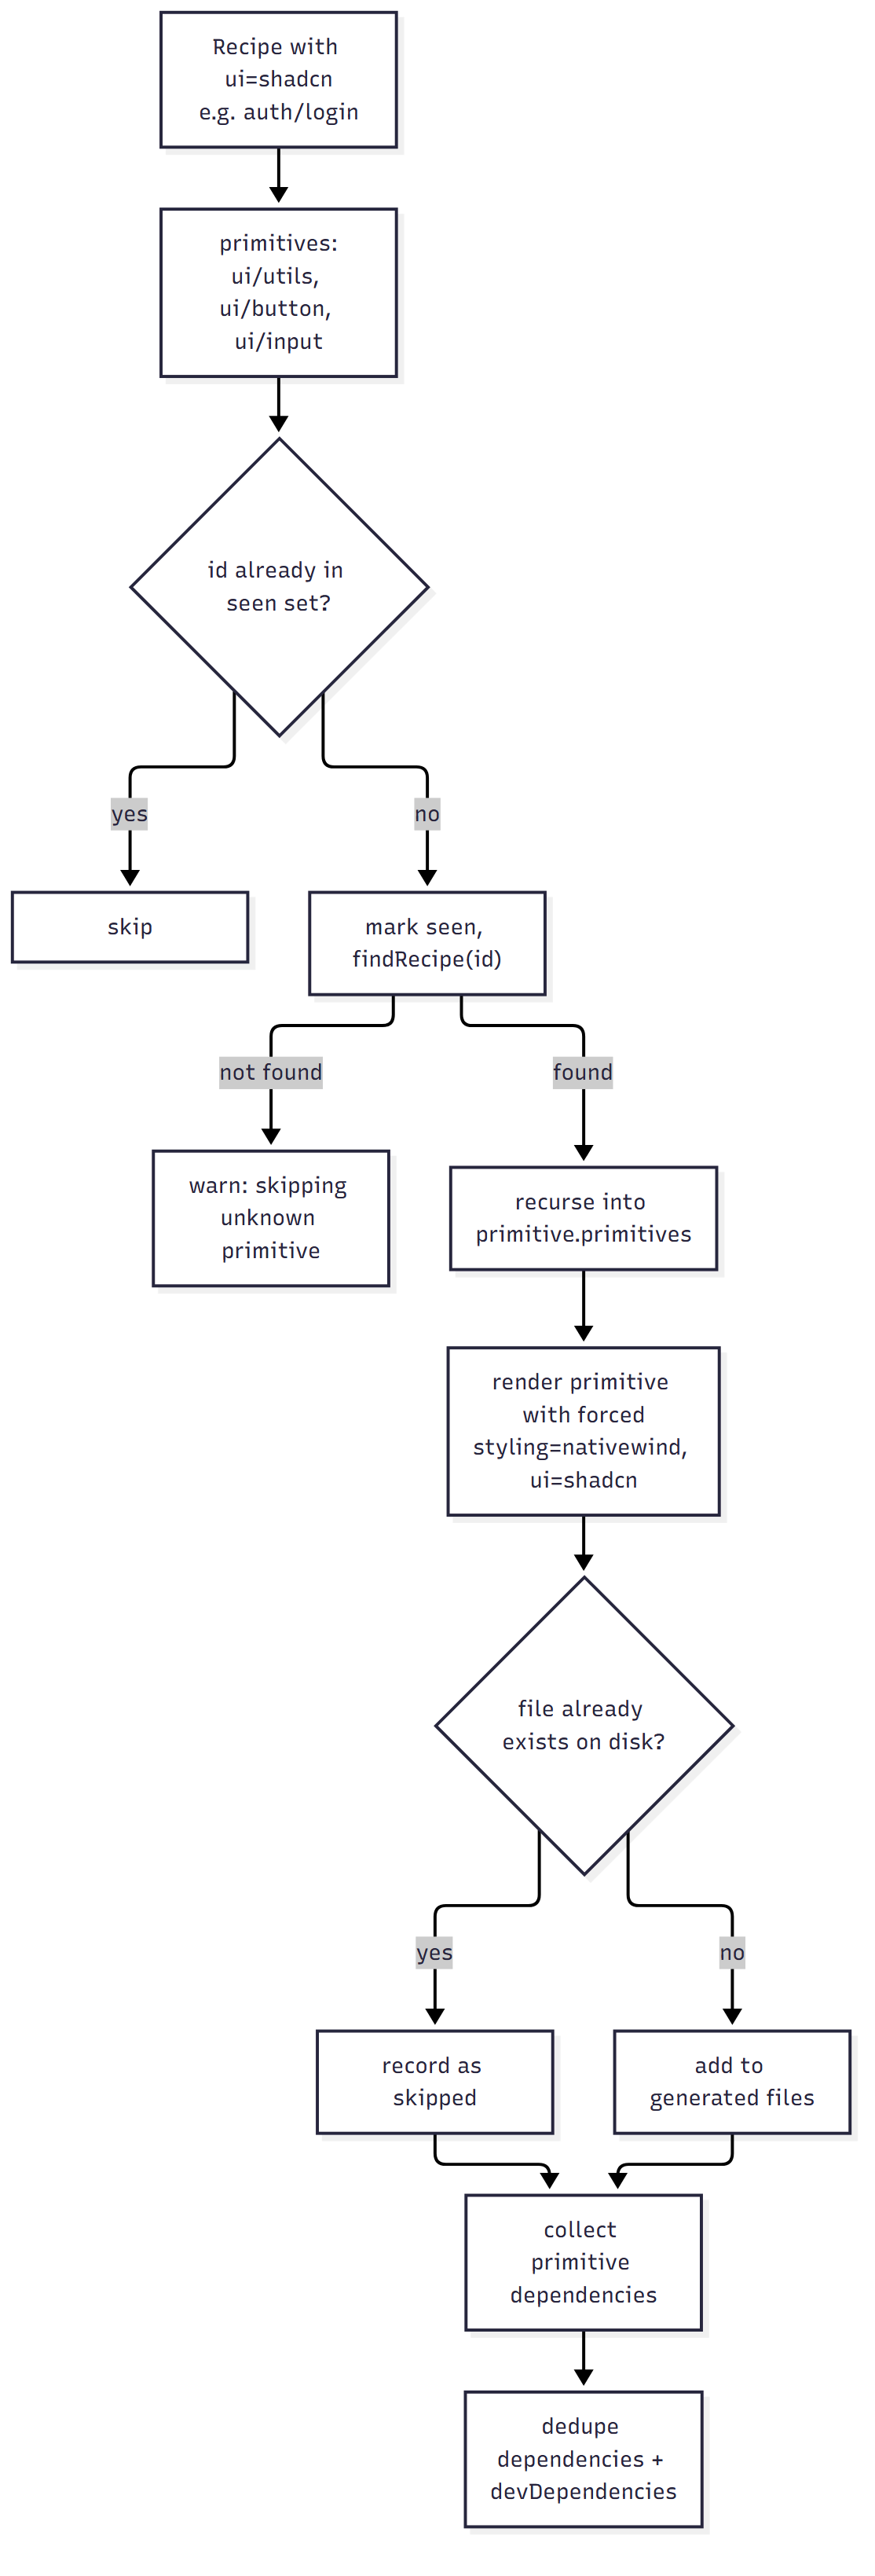
\includegraphics[width=0.95\textwidth]{diagrams/primitive-resolution.png}
\caption{Recursive UI primitive resolution when \texttt{ui=shadcn}}
\label{fig:primitive-resolution}
\end{figure}

\section{\texttt{expo-snippets} --- VS Code extension}

\begin{longtable}{p{4.2cm}p{9.8cm}}
\caption{Extension functions}\\
\toprule
\textbf{Function} & \textbf{Behaviour} \\
\midrule

\texttt{activate(context)} & Registers commands and the completion provider, creates
a right-aligned status bar item (\texttt{\$(sparkle) Expo Snips}) bound to
\texttt{expo-snips.addScreen}, and pushes it to subscriptions. \\
\texttt{deactivate()} & Empty. \\
\texttt{registerCommands(context)} & Registers \texttt{expo-snips.addScreen}
(index Quick Pick, with an ``Open Settings'' error action when the catalog is
empty) and \texttt{expo-snips.generateFromCompletion(recipeId?)}. \\
\texttt{registerCompletionProvider(context)} & Language-filtered provider triggered on
\texttt{:}; tests the line prefix against \texttt{/expo-snips:\$|snip:\$/};
returns items whose \texttt{insertText} is empty and whose command carries the
recipe id. \\
\texttt{pickSupported(supported, preferred, fallback)} & Returns the preferred value
when supported, otherwise the first supported value, otherwise the fallback. \\
\texttt{resolveOptions(recipe, detected)} & Reads the four default settings and the
language; applies \texttt{pickSupported}; enforces shadcn constraints. \\
\texttt{pickVariant(recipe)} & Returns undefined when no variants; otherwise a Quick
Pick of variant labels. \\
\texttt{detectPackageManager(dir)} & Same lockfile probes as the CLI. \\
\texttt{installDependencies(dir, deps, devDeps)} & Creates and reveals an ``Expo
Snips'' terminal and sends \texttt{add} commands. \\
\texttt{generateScreen(recipe)} & Resolves the workspace root, detects the project,
resolves options and variant, renders, writes files under a progress notification,
resolves primitives, upserts the manifest, shows an information message with an
``Open main file'' action, and installs dependencies when enabled. \\
\texttt{getWorkspaceRoot()} & Returns the first workspace folder's filesystem path. \\
\bottomrule
\end{longtable}

\textbf{Behavioural difference from the CLI.} The extension never prompts for
styling, router, UI or icons --- it silently selects from the detected values and
the configured defaults. The CLI prompts. This is the single largest behavioural
divergence between the two surfaces.

\section{State}

\begin{longtable}{p{3.4cm}p{4.4cm}p{6.2cm}}
\caption{State inventory}\\
\toprule
\textbf{State} & \textbf{Location} & \textbf{Lifetime} \\
\midrule

Remote index cache & \texttt{registry.ts} (extension) & Process; 5 minutes
(\texttt{CACHE\_TTL\_MS}). \\
Registry back-off timestamp & \texttt{remoteRetryAfter} (extension) & Process; 5
minutes after a failed fetch. \\
Embedded catalog maps & \texttt{localRecipes}, \texttt{localById} (both clients) &
Module lifetime. \\
Generation context & Function local (\texttt{add.ts}, \texttt{generator.ts}) & Single
generation. \\
Manifest & \texttt{.expo-snips.json} on disk & Permanent until deleted. \\
Generated files & The user's project & Permanent. \\
\bottomrule
\end{longtable}

No global mutable state exists in the CLI. The extension holds the two cache
variables above at module scope.

\section{Data access patterns}

\begin{itemize}
  \item \textbf{Reads:} \texttt{fs.readJSON} / \texttt{fs.existsSync} /
        \texttt{fs.pathExists} for project detection and manifest reads;
        \texttt{fs.readFileSync} for diff comparison; \texttt{fetch} for the remote
        registry.
  \item \textbf{Writes:} \texttt{fs.ensureDir} + \texttt{fs.writeFile} for generated
        files; \texttt{fs.writeJSONSync} for the manifest.
  \item \textbf{Catalog access:} synchronous filesystem reads in
        \texttt{@expo-snips/registry} (build-time only) and in-memory lookups in the
        clients.
\end{itemize}

There is no transaction semantics, no locking and no atomic write;
\texttt{writeFile} overwrites in place.

\section{Dependencies between modules}

\begin{table}[H]
\centering
\caption{Module-level import graph (workspace)}
\begin{tabular}{p{5.4cm}p{8.2cm}}
\toprule
\textbf{Module} & \textbf{Imports from workspace} \\
\midrule
\texttt{core/src/*} & none \\
\texttt{cli/src/commands/*} & \texttt{@expo-snips/core}, \texttt{../utils/*} \\
\texttt{cli/src/utils/*} & \texttt{@expo-snips/core}, \texttt{./generated/registry-data} \\
\texttt{registry/src/index.ts} & \texttt{@expo-snips/core} \\
\texttt{vscode-extension/src/*} & \texttt{@expo-snips/core}, \texttt{./generated/registry-data} \\
\bottomrule
\end{tabular}
\end{table}
